\chapter{Design del Protocollo}
\label{chap:design_protocollo}
\section{Architettura generale del sistema}
\begin{figure}[H]
    \centering
    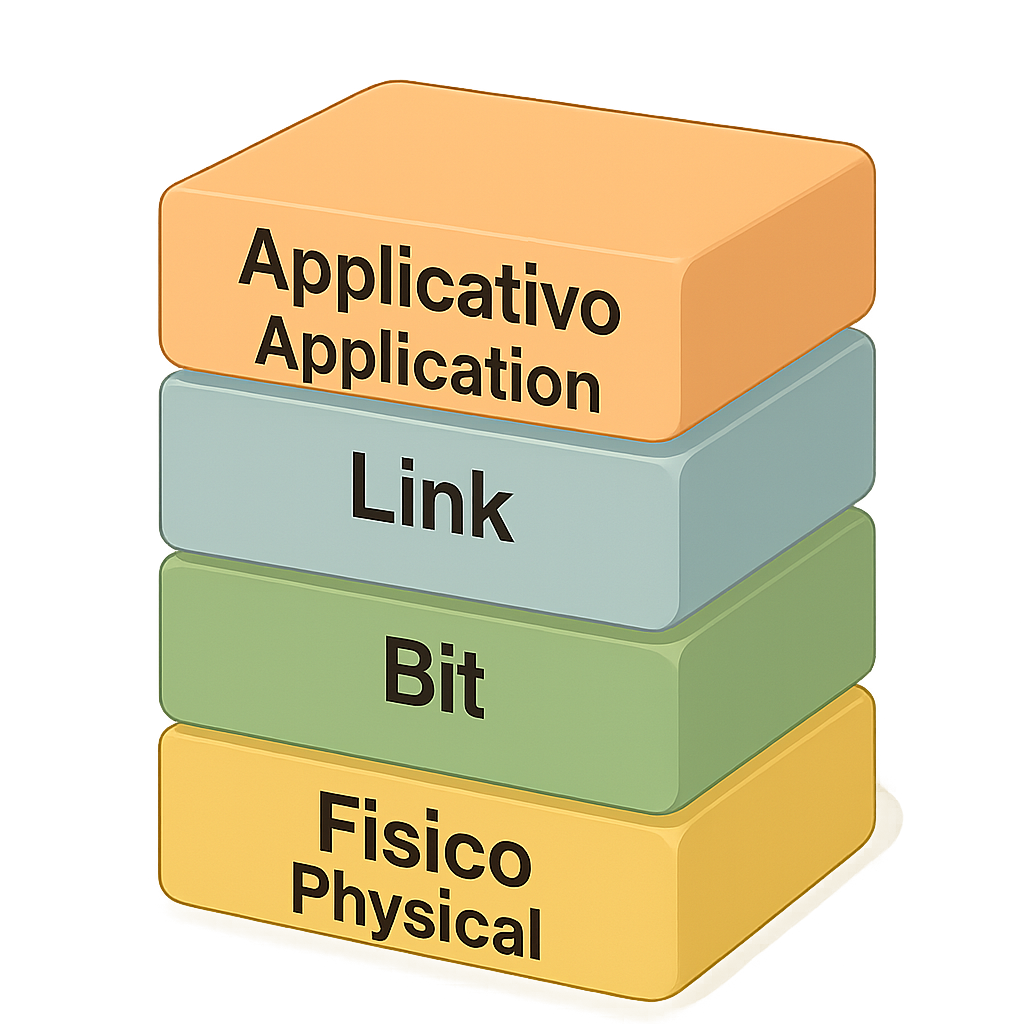
\includegraphics[width=0.35\textwidth]{immagini/layers.png}
    \caption{Livelli del Protocollo}
    \label{fig:layers}
\end{figure}
Il protocollo è strutturaro in quattro livelli principali, ognuno con una funzione specifica.
\section{Livello Fisico}
\label{sec:livello_fisico}
Il livello fisico è responsabile della tramissione dei bit precedentemente composti dal livello Bit.
Questo sfrutta uno speaker per la trasmissione e un microfono per la ricezione dei bit che vengono trasmessi mediante coppie superimposte di frequenze.
\subsection{Ingresso}
\label{sec:ingresso_livello_fisico}
Il microfono I2S (descritto nel \autoref{chap:implementazione_hardware}) è collegato al microcontrollore ESP32 tramite il bus I2S, sfruttando uno dei due canali disponibili.  
Il segnale audio viene campionato a $48\,\text{kHz}$ con una risoluzione di 16 bit, per poi essere gestito mediante due array in swapping, concetto che verrà approfondito successivamente. \\

\noindent
La scelta della frequenza di campionamento deriva dal \textbf{teorema di Nyquist-Shannon} \citep{shannon1949}, secondo il quale un segnale può essere ricostruito senza ambiguità se la frequenza di campionamento $f_s$ è almeno doppia rispetto alla massima frequenza del segnale $f_{\max}$:
\[
f_s \geq 2 f_{\max}.
\]
Ne consegue che la massima frequenza rappresentabile è
\[
f_{\text{Nyquist}} = \frac{f_s}{2}.
\]

Nel nostro caso:
\[
f_s = 48\,\text{kHz} \quad \Rightarrow \quad f_{\text{Nyquist}} = 24\,\text{kHz}.
\]

Poiché l’orecchio umano percepisce frequenze fino a circa $20\,\text{kHz}$ \citep{zwicker1999psychoacoustics}, la scelta di $48\,\text{kHz}$ garantisce la copertura dell’intero spettro udibile, con un margine di sicurezza di $4\,\text{kHz}$. Frequenze prossime al limite teorico di Nyquist risulterebbero invece difficili da catturare senza aliasing, a causa dei limiti pratici dei filtri anti-alias. \\

\noindent
Per l’elaborazione, i campioni vengono raccolti in blocchi di lunghezza $N = 512$. Con la frequenza di campionamento fissata:
\[
T_{\text{blocco}} = \frac{N}{f_s} = \frac{512}{48 \cdot 10^3} \approx 0.01066\,\text{s}.
\]
Ogni blocco di dati rappresenta quindi un intervallo di circa $10.7\,\text{ms}$ di segnale audio.  
Questa durata, successivamente a una attenta analisi effettuata sul software Audacity, si è rivelata sufficiente per poter catturare in modo affidabile i toni.
\begin{figure}[H]
    \centering
    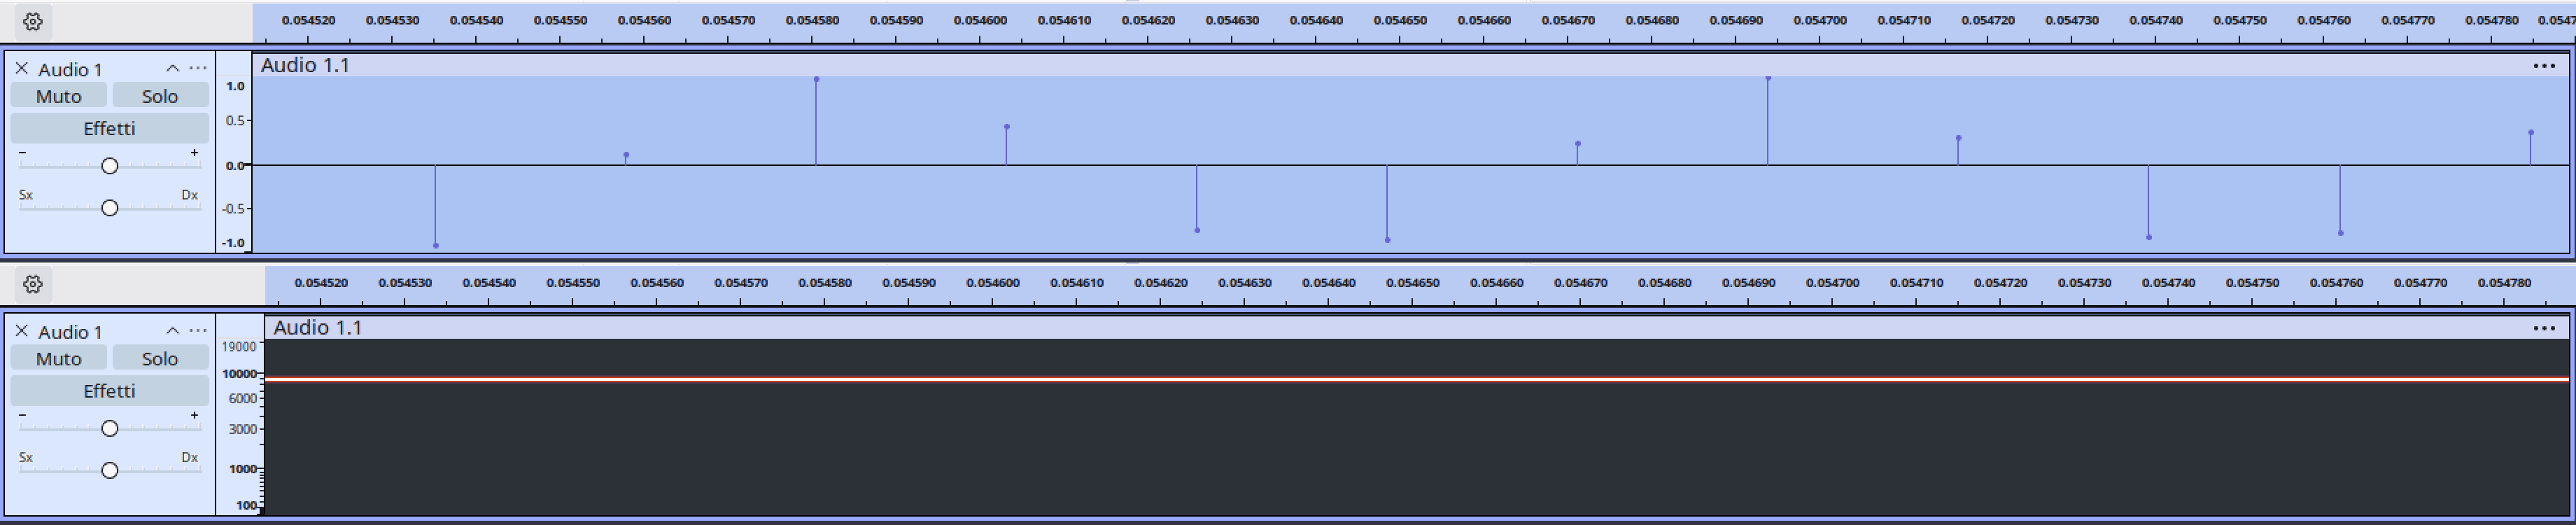
\includegraphics[width=0.9\textwidth]{immagini/audacity_spectrum.png}
    \caption{Verifica della cattura del tono a 9kHz con campionamento a 48kHz nel periodo 0-0.010 secondi, utilizzando finestra di Hann su 512 elementi}.
    \label{fig:spettro_audacity}
\end{figure}


\paragraph{}
\label{par: fft_calcolo}
\noindent
Una volta acquisito il blocco, viene calcolata la \textbf{trasformata veloce di Fourier (FFT)} \citep{cooley1965fft} per analizzare lo spettro in frequenza. La complessità della FFT cresce come $N \log_2 N$, e per $N=512$ si hanno circa:
\[
512 \cdot \log_2(512) = 512 \cdot 9 = 4608
\]
operazioni complesse.  

Sul microcontrollore ESP32 \citep{esp32techref}, operante a $120\,\text{MHz}$, questo si traduce in un tempo di elaborazione di circa $0.42\,\text{ms}$ per blocco, ovvero $\sim 0.83\,\mu\text{s}$ per campione. In termini di carico computazionale: $\sim 20$ moltiplicazioni, $\sim 29$ addizioni/sottrazioni e un’operazione di radice quadrata per campione, pari a $\sim 99$ cicli di clock.  

\noindent
Questo significa che, a fronte di una finestra temporale di $10.7\,\text{ms}$, l’FFT viene calcolata in meno del $5\%$ del tempo disponibile, consentendo un’elaborazione in tempo reale anche senza multi-threading.

\begin{figure}[H]
    \centering
    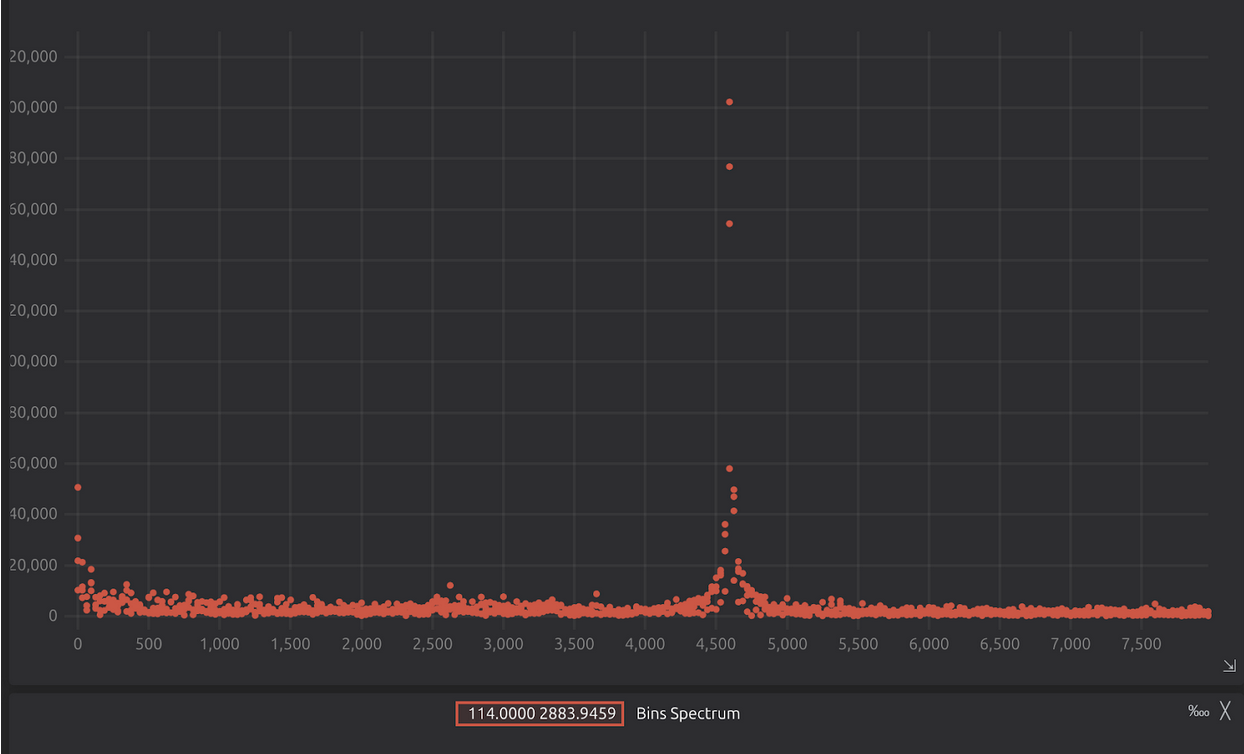
\includegraphics[width=0.65\textwidth]{immagini/fft_spectrum.png}
    \caption{Grafico contentente lo spettro di frequenza calcolato tramite FFT} su un blocco di $512$ campioni acquisiti a $48\,\text{kHz}$.
    \label{fig:spettro}
\end{figure}

\paragraph{FFT, bin e asse delle frequenze}
L'algoritmo FFT non calcola direttamente lo spettro in frequenza continua, bensì restituisce $N$ valori discreti $X[k]$ detti \emph{bin}, con indici
\[
k=0,1,\dots,N-1.
\]
Questi bin rappresentano i coefficienti della trasformata discreta e contengono l’informazione spettrale su griglie di frequenza equispaziate. 
Per $N=512$ e frequenza di campionamento $F_s=48~\mathrm{kHz}$, ciascun bin corrisponde alla frequenza
\[
f_k \;=\; k\,\frac{F_s}{N},
\qquad \Delta f = \frac{F_s}{N} = \frac{48\,000}{512} = 93.75~\mathrm{Hz}.
\]
Dunque l’asse $x$ del grafico, che mostra le frequenze in Hz, è in realtà una \emph{ridenominazione} dei bin calcolati dall’FFT. 
Ogni valore sull’asse delle ascisse non è una misura continua, ma la mappatura del bin discreto $k$ nella corrispondente frequenza $f_k$.

\paragraph{Simmetria dello spettro}
Poiché il segnale è reale, vale la simmetria
\[
X[N-k] = \overline{X[k]} \quad \Rightarrow \quad |X[N-k]|=|X[k]|.
\]
Per questo motivo lo spettro viene spesso mostrato soltanto fino al bin $N/2$, ossia da $k=0$ a $k=256$. 
In particolare, il bin $k=256$ corrisponde alla frequenza massima non ambigua, cioè la frequenza di Nyquist:
\[
f_{256} = 256 \cdot \frac{48\,000}{512} = 24~\mathrm{kHz}.
\]

Durante la creazione di questo protocollo sono emerse diverse difficoltà legate alla presenza di rumore ambientale,
questa condizione ha reso necessario l'uso di tecniche di filtraggio.

\subsubsection{Filtraggio e riconoscimento dei toni}
\label{subsec:filtraggio}

Una parte cruciale del processo di design del protocollo è stata la scelta delle frequenze da utilizzare per la trasmissione dei dati. 
I picchi che vengono selezionati dalla fase di filtraggio devono appartenere a un insieme di frequenze predefinite, così da poter essere riconosciuti dal \textbf{Livello Bit}. \\ 
La seguente tabella riporta l’insieme delle frequenze adottate, distinguendo quelle di tipo \emph{carrier} da quelle destinate al trasferimento dei dati:

\begin{table}[H]
    \centering
    \begin{tabular}{c c}
        % --- prima tabella ---
        \begin{tabular}{|c|c|}
        \hline
        \textbf{Frequenza [Hz]} & \textbf{Tipo} \\
        \hline
        1000  & \cellcolor{red!50} Carrier \\
        \hline
        1400  & \cellcolor{yellow!50} Data \\
        \hline
        1800  & \cellcolor{yellow!50} Data \\
        \hline
        2200  & \cellcolor{yellow!50} Data \\
        \hline
        2600  & \cellcolor{yellow!50} Data \\
        \hline
        3000  & \cellcolor{yellow!50} Data \\
        \hline
        3400  & \cellcolor{yellow!50} Data \\
        \hline
        3800  & \cellcolor{yellow!50} Data \\
        \hline
        4200  & \cellcolor{yellow!50} Data \\
        \hline
        4600  & \cellcolor{yellow!50} Data \\
        \hline
        5000  & \cellcolor{yellow!50} Data \\
        \hline
        \end{tabular}
        &
        \hspace{0.5cm} % <-- spazio in mezzo
        % --- seconda tabella ---
        \begin{tabular}{|c|c|}
        \hline
        \textbf{Frequenza [Hz]} & \textbf{Tipo} \\
        \hline
        5400  & \cellcolor{yellow!50} Data \\
        \hline
        5800  & \cellcolor{yellow!50} Data \\
        \hline
        6200  & \cellcolor{yellow!50} Data \\
        \hline
        6600  & \cellcolor{yellow!50} Data \\
        \hline
        7000  & \cellcolor{yellow!50} Data \\
        \hline
        7400  & \cellcolor{yellow!50} Data \\
        \hline
        7800  & \cellcolor{yellow!50} Data \\
        \hline
        8200  & \cellcolor{yellow!50} Data \\
        \hline
        8600  & \cellcolor{red!50} Carrier \\
        \hline
        9000  & \cellcolor{red!50} Carrier \\
        \hline
              & \cellcolor{white!50}      \\
        \hline
        \end{tabular}
    \end{tabular}
    \caption{Frequenze e tipi di segnale}
    \label{tab:frequenze}
    \end{table}
    

Il filtraggio avviene nel dominio della frequenza, dopo l’applicazione della trasformata FFT a 512 punti.
 A differenza dei filtri digitali convenzionali (IIR/FIR), la selezione dei toni non si basa su maschere statiche ma su un insieme di procedure che rendono il sistema adattivo al rumore e preciso nell’identificazione dei picchi. 
 Inizialmente, quando il protocollo era ancora nelle sue fasi embrionali, era stato deciso di utilizzare una semplice soglia fissa (filtro passa-basso) per discriminare i picchi delle frequenze predefinite dal rumore. 
 Questa soluzione, tuttavia, si è rivelata inefficace: i microfoni presentano una risposta in frequenza che degrada sulle alte frequenze, rendendo i livelli in dB di queste ultime attenuati al punto da non superare la soglia prefissata. 
 Inoltre, il rumore ambientale non è mai costante ma varia nel tempo e nello spettro, il che rendeva difficile definire un limite statico in grado di funzionare in tutte le condizioni.\\

In un’evoluzione successiva si è quindi ipotizzato l’impiego di soglie fisse ma differenziate per ciascuna frequenza, così da compensare la risposta non piatta del microfono. \\
 Per calcolare tali soglie è stato utilizzato un algoritmo di regressione lineare, in grado di stimare la retta che meglio approssima l’andamento della soglia minima:
\[
y = \beta_{} + \beta_{}x + \varepsilon \rightarrow y = -301.751324 \times x + 48531.689491
\]
dove $x$ rappresenta il numero del bin. La \autoref{fig:spettro2} mostra lo spettro in frequenza di tre toni (basso, medio e alto) e mette in evidenza l’attenuazione introdotta dalla risposta del microfono.
\begin{figure}[H]
    \centering
    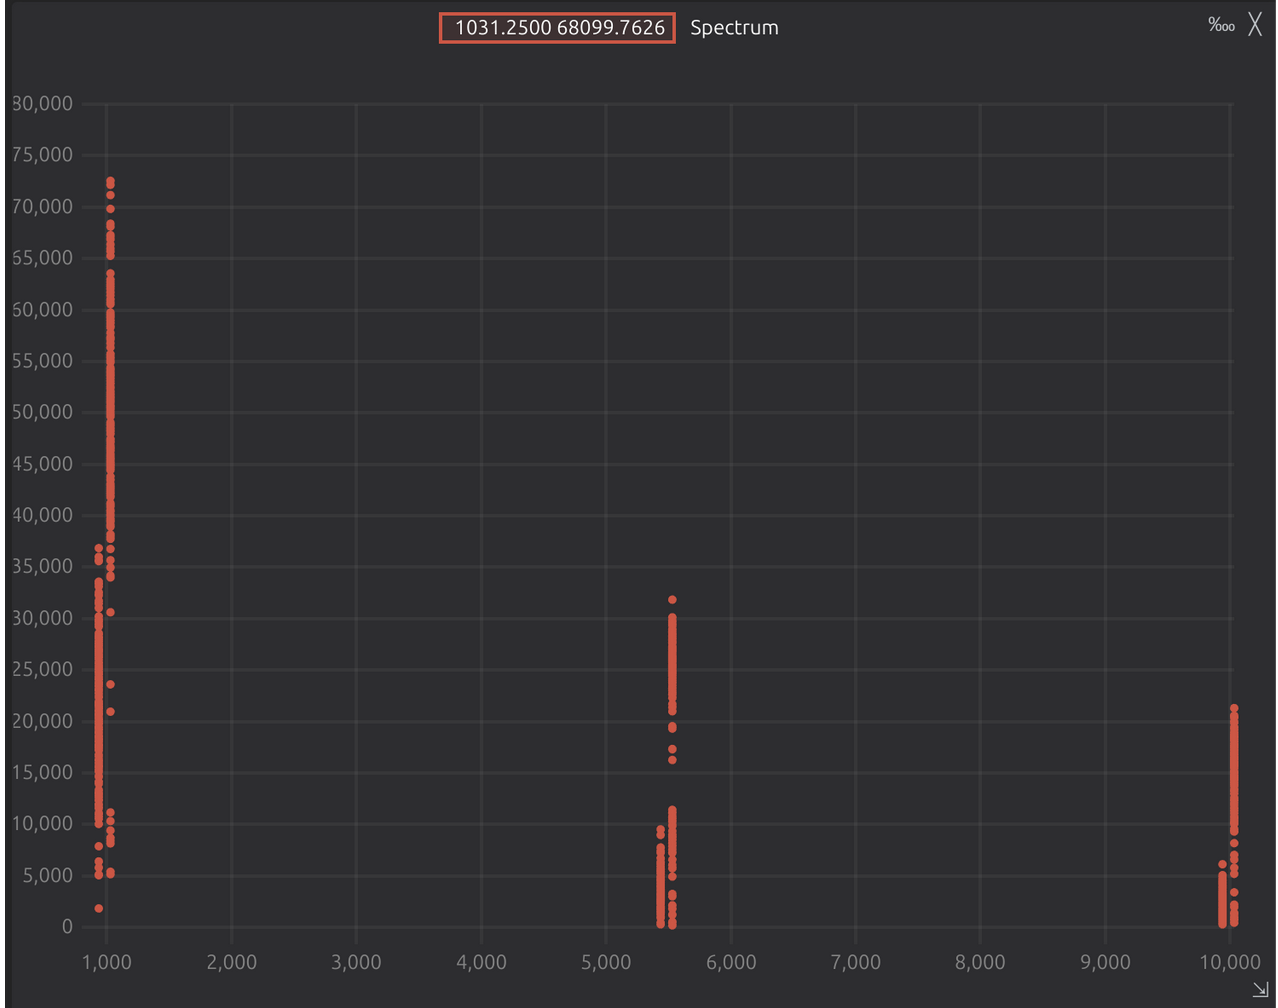
\includegraphics[width=0.65\textwidth]{immagini/fft_regression_check.png}
    \caption{Grafico contenente lo spettro di frequenza di tre frequenze (bassa, media, alta), utilizzato per identificare l'attenuazione in frequenza del microfono.}
    \label{fig:spettro2}
\end{figure}

Il sistema attuale ha superato queste limitazioni introducendo una catena di elaborazione più robusta.
 In primo luogo viene stimato il livello medio di rumore calcolando la media delle ampiezze spettrali:
\[
\text{noise\_floor} = \frac{1}{N}\sum_{k=0}^{N-1} |X[k]|
\]
dove $X[k]$ è il modulo del $k$-esimo bin. A partire da questa misura viene definita una soglia dinamica, 
proporzionale al rumore, che permette di adattarsi alle condizioni del segnale: un picco viene considerato 
valido solo se la sua ampiezza supera di almeno otto volte il livello medio di rumore. Per ridurre ulteriormente 
i falsi positivi, ogni frequenza candidata deve corrispondere a un \textbf{massimo locale}, ossia il \textbf{bin identificato}
 deve avere ampiezza superiore rispetto ai sei \textbf{bin adiacenti a sinistra e a destra}. \\
 \begin{figure}[H]
    \centering
    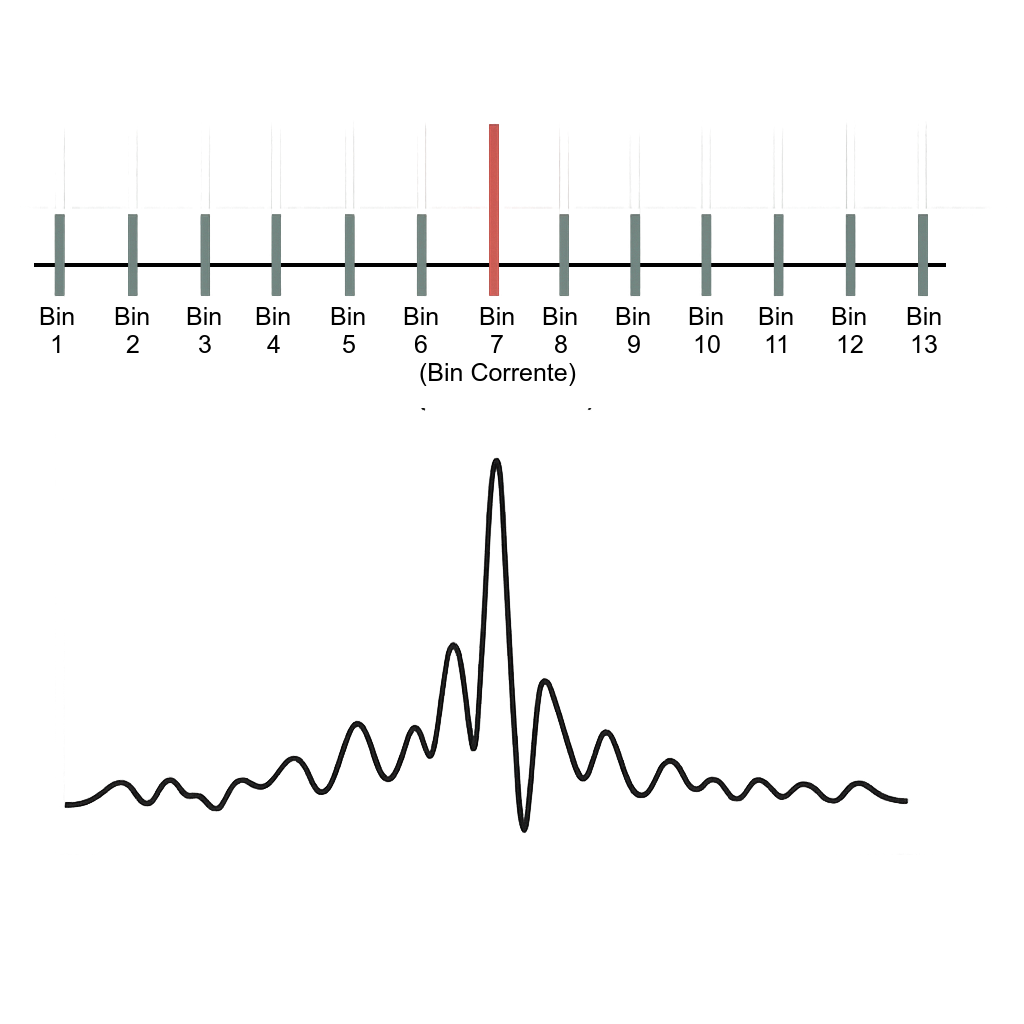
\includegraphics[width=0.5\textwidth]{immagini/local_peak.png}
    \caption{Picco Locale nell'intorno dei sei Bins}
    \label{fig:bins_local_peak}
\end{figure}
\paragraph{Interpolazione parabolica}
\label{par: interpolazione_parabolica}
 A questo punto, per migliorare 
 la risoluzione in frequenza oltre i limiti del singolo bin FFT, viene applicata un’\textbf{interpolazione parabolica} basata
  sui valori $X[k-1]$, $X[k]$ e $X[k+1]$, secondo la formula
\[
p = \tfrac{1}{2}\,\frac{\alpha - \gamma}{\alpha - 2\beta + \gamma},
\]
dove $\alpha = |X[k-1]|$, $\beta = |X[k]|$ e $\gamma = |X[k+1]|$. La frequenza stimata diventa così $f_k + p\,\Delta f$, con $\Delta f = 93.75\,\text{Hz}$, 
ottenendo una risoluzione sub-bin.\\ 
\begin{figure}[H]
    \centering
    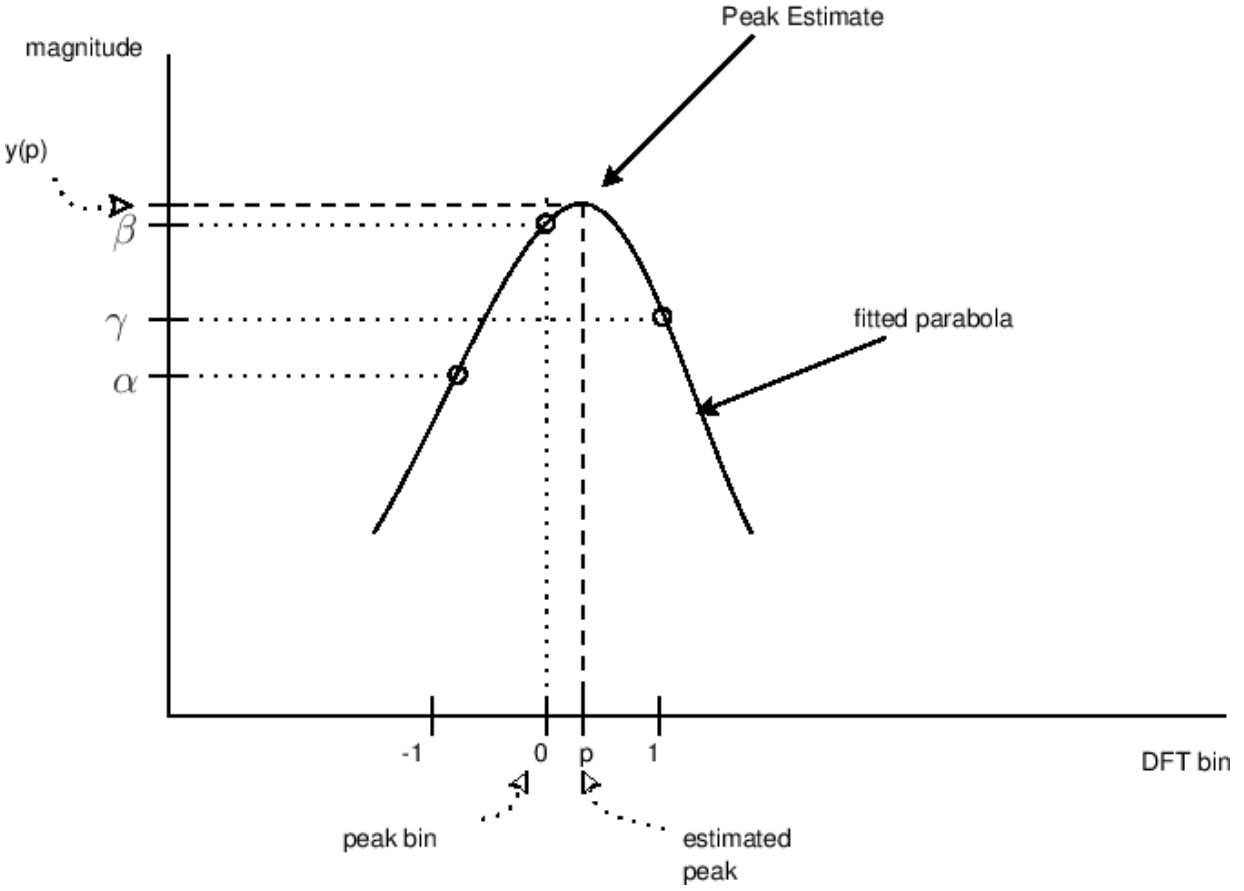
\includegraphics[width=0.5\textwidth]{immagini/parabolic_interpolation.png}
    \caption{Interpolazione Parabolica \citep{QuadraticInterpolationSpectralPeaks}}
    \label{fig:interpolazione_parabolica}
\end{figure}
È inoltre disponibile, sebbene disattivato di default, un modulo di regressione lineare che consente di compensare eventuali 
pendenze dello spettro in condizioni particolarmente critiche. Infine, i \textbf{picchi confermati vengono incapsulati in una struttura dati (\texttt{struct\_tone\_frequencies})
 e inoltrati al \emph{Livello Bit}}, che li utilizza per ricostruire i bit associati ai canali \emph{master}, \emph{slave} e \emph{config}.
\subsection{Uscita}
\label{sec:uscita_livello_fisico}
Il livello fisico si occupa anche della trasmissione dei dati, convertendo coppie di frequenze ricevute dal Livello Bit in segnali audio.
Questa operazione viene eseguita mediante la sintesi digitale di due toni sinusoidali, che vengono sommati, sistemati in fase, sistemati in ampiezza
ed infine inviati attraverso il bus I2S ad un amplificatore di potenza (descritto nel \autoref{chap:implementazione_hardware}).

\paragraph{Sintesi dei toni}
L'emissione di una coppia di frequenze superimposte è un operazione che coinvole l'utilizzo di diverse tecniche di sintesi digitale.\\
In primo luogo viene calcolato il numero necessario di campioni che comporanno la \textbf{sinusoide}, 
per far ciò è necessario utilizzare la stessa frequenza di campionamento adottata per l'acquisizione, ovvero $48\,\text{kHz}$, ed la durata d'emissione che
è stata fissata a $0.024\,\text{s}$.
La scelta di questa durata deriva dalla finestra temporale di $10.7\,\text{ms}$ utilizzata per l'analisi FFT, quindi $24\,\text{ms}$ 
è un compromesso che consente di avere un segnale sufficientemente lungo per essere percepito e demodulato, evitando cosi che \textbf{la finestra di ascolto (FFT)}
possa essere in mezzo tra un tono e l'altro, rendendo cosi difficile la demodulazione.
Con questa durata, quindi, si avrà sempre una serie di 512 campioni in ingresso che conterranno, sicuramente, i toni.\\

Il numero di campioni necessari per la sintesi è quindi 
\begin{equation}
    N = f_s \cdot T
    \end{equation}
    
    \begin{equation}
    N = 48\,000 \,\text{Hz} \cdot 0.024 \,\text{s} = 1152 \,\text{campioni}
    \end{equation}

    \begin{figure}[H]
        \centering
        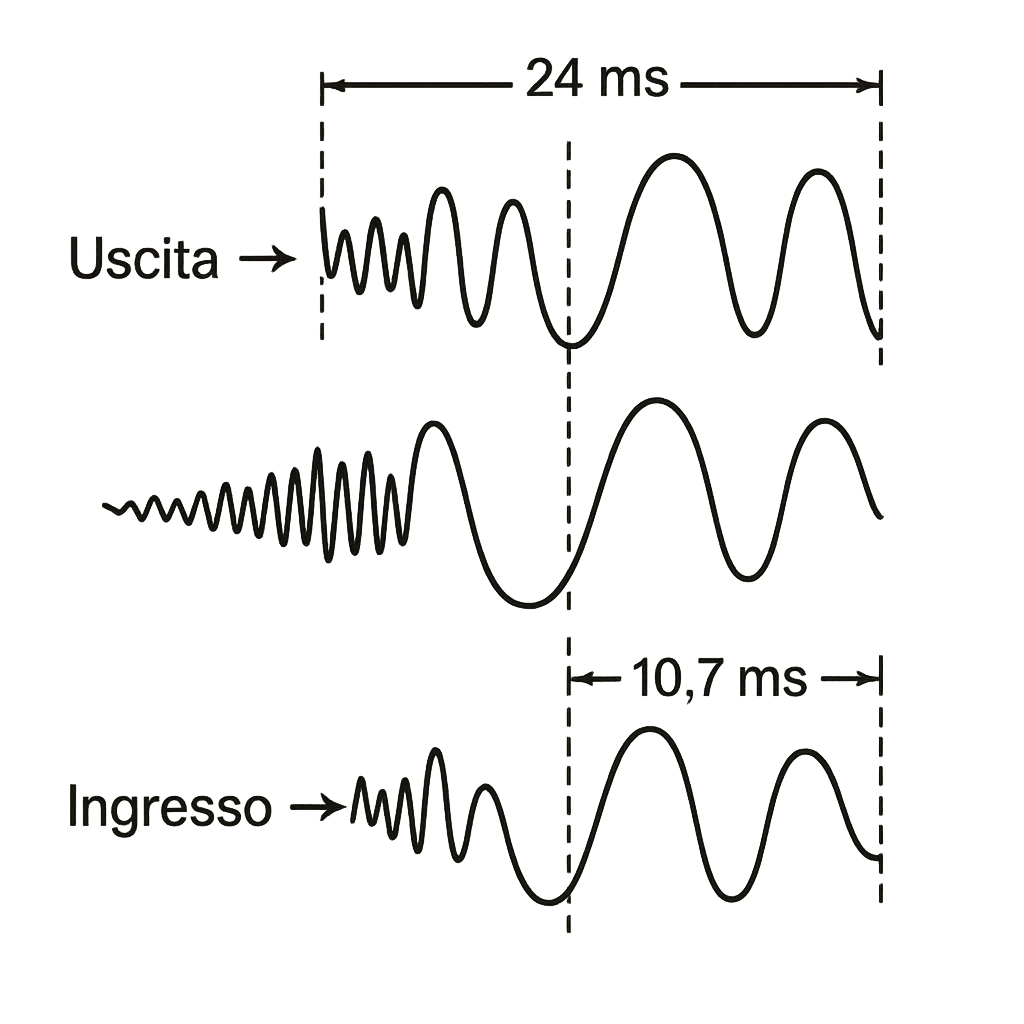
\includegraphics[width=0.5\textwidth]{immagini/window_listening.png}
        \caption{Finestra d'ascolto della FFT sul segnale emesso}
        \label{fig:finestra_ascolto}
    \end{figure}

A seguito di diversi test, dove è stato riscontrato un "fruscio" tra l'emissione di un tono e l'altro,
 è stato implementato un sistema di allineamento di fase. \\
Questo funziona attraverso una variabile che tiene traccia della fase dell'ultimo campione emesso,
 in questo modo il primo campione del nuovo tono sarà sempre in fase con l'ultimo campione del tono precedente.
 Ciò consente di evitare discontinuità nel segnale che si traducono in rumore udibile.\\
 La sintesi di ciascuna sinusoide avviene quindi secondo la formula
\begin{equation}
    x[n] = A \cdot \frac{\sin(\phi_1)+\sin(\phi_2)}{2}
\end{equation}
formula semplificata dove $A$ è l'ampiezza del segnale, $\phi_1$ e $\phi_2$ sono le fasi delle due sinusoidi calcolate come 
\begin{equation}
    \phi = \frac{2 \pi f}{f_s}
\end{equation}

\section{Livello Bit}
\label{sec:livello_bit}
Il Livello Bit si occupa di convertire le frequenze ricevute dal Livello Fisico in bit, e viceversa.
Il pacchetto con cui il livello Bit comunica con il Livello Fisico è la seguente struttura dati 

\definecolor{lightgray}{RGB}{235,235,235}
\definecolor{white}{RGB}{255,255,255}


\begin{table}[H]
\centering
\label{tab:master_slave_config}
\resizebox{\textwidth}{!}{%
\begin{tabular}{
|>{\columncolor{white}}c
|>{\columncolor{white}}c
|>{\columncolor{white}}c|
>{\columncolor{lightgray}}c
|>{\columncolor{lightgray}}c
|>{\columncolor{lightgray}}c|
>{\columncolor{white}}c
|>{\columncolor{white}}c
|>{\columncolor{white}}c|
}
\hline
\multicolumn{3}{|c|}{\cellcolor{white} Master} &
\multicolumn{3}{c|}{\cellcolor{lightgray} Slave} &
\multicolumn{3}{c|}{\cellcolor{white} Config} \\
\hline
Frequenza 1 & Frequenza 2 & Frequenza 3 &
Frequenza 1 & Frequenza 2 & Frequenza 3 &
Frequenza 1 & Frequenza 2 & Frequenza 3 \\
\hline

\end{tabular}
}
\caption{Struttura di comunicazione tra Livello Bit e Livello Fisico}
\end{table}

Ogni gruppo (master, slave, config) rappresenta un gruppo a sè stante, che può essere utiilizzato per diversi scopi, 
questo avviene al fine di evitare conflitti tra i nodi, in quanto il ruolo è già indicato dalle frequenze che usano.
Il livello Fisico quindi restituisce per ogni gruppo una struttura dati contenente 2 frequenze, se le 3 frequenze fossero tutte presenti allo stesso momento si avrebbe,
allo stato attuale della tecnologia un errore Multi-Tone.
In ogni gruppo, le frequenze seguono una logica definita come segue:
\begin{itemize}
\item La prima frequenza rappresenta quale \textbf{Signal Code} utilizzare dal lato sinistro della tabella che segue
\item La seconda frequenza è la portante ed è sempre la stessa per ogni gruppo, questa serve successivamente per la decodifica
\item La terza frequenza rappresenta quale \textbf{Signal Code} utilizzare dal lato destro della tabella che segue
\end{itemize}



    \begin{table}[H]
    \centering
    \label{tab:freq_codici}
    \resizebox{\textwidth}{!}{%
    \begin{tabular}{|l|>{\columncolor{lightgray}}l|l|>{\columncolor{lightgray}}l|}
    \hline
    \textbf{Frequenza} & \textbf{Signal Code} & \textbf{Portante} & \textbf{Signal Code} \\
    \hline
    1000 & & Master Carrier & \\
    1400 & (0) Bits: 0 & & \\
    1800 & (1) Bits: 00 & & \\
    2200 & (2) Bits: 000 & & \\
    2600 & (3) Bits: 0000 & & \\
    3000 & (4) Bits: 00000 & & \\
    3400 & (5) Bits: 000000 & & \\
    3800 & (6) Bits: 0000000 & & \\
    4200 & (7) Bits: 0000000 0000000 & & \\
    4600 & (8) Bits: 0000000 0000000 000000 & & \\
    5000 & & & (9) Bits: 1 \\
    5400 & & & (10) Bits: 11 \\
    5800 & & & (11) Bits: 111 \\
    6200 & & & (12) Bits: 1111 \\
    6600 & & & (13) Bits: 11111 \\
    7000 & & & (14) Bits: 111111 \\
    7400 & & & (15) Bits: 1111111 \\
    7800 & & & (16) Bits: 1111111 1111111 \\
    8200 & & & (17) Bits: 1111111 1111111 111111 \\
    8600 & & Config Carrier & \\
    9000 & & Slave Carrier & \\
    \hline
    \end{tabular}
    }
    \caption{Mappatura frequenze, codici e portanti}
    \end{table}


L'utilizzo di questo schema di codifica, viene dopo l'esecuzione di diversi test, in quanto in origine i dati venivano trasmessi utilizzando 3 frequenze per ogni gruppo:
\begin{itemize}
\item La prima frequenza rappresentava se era uno 0
\item La seconda frequenza era la portante
\item La terza frequenza rappresentava se era un 1
\end{itemize}
L'utilizzo della \autoref{tab:freq_codici} ha permesso di comprimere i pacchetti di dati a livello di bit, in quanto ora è possibile trasmettere più bit
 con una sola frequenza.\\
Questo ha permesso di aumentale la velocità di trasmissione fino a 5[codes per second],che nel caso più favorevole rappresentano \textbf{30bps}, 
che seppur bassa è comunque un miglioraremento rispetto alla versione precedente che raggiungeva al massimo 5bps.\\
Inoltre, grazie a questa codifica, è possibile trasmettere il codice 8 (21 volte 0) 
con estrema facilità, questo corrisponde alla ripetizione del carattere ASCII NUL per tre volte, che, nel protocollo corrisponde all' End of Packet (EOP).\\

\subsection{Decodifica}
In fase di decodifica, come preannunciato, il Livello Bit riceve dal Livello antecedente una struttura dati contenente fino a 2 frequenze per ogni gruppo (master, slave, config).
Questo associa la frequenza data al corrispondente \textbf{Signal Code}, attraverso
\begin{equation}
s[n] = \frac{f-base}{step} = \frac{f-1000}{400}
\end{equation}
Dove \texttt{base} è la frequenza minima (1000Hz), \texttt{step} è la differenza tra una frequenza e l'altra (400Hz) e \texttt{f} è la frequenza ricevuta.

Questo permette di ottenere il \textbf{Signal Code} che può essere compreso tra 0 e 17, che viene successivamente convertito in bit attraverso
la \autoref{tab:freq_codici}.\\
Durante la fase di conversione tra Signal Code e bit, nel momento in cui viene identificato il Codice 8 (21 volte 0) viene interpretato come End of Packet (EOP),
avviene quindi la \textbf{memorizzazione del pacchetto in bits nell'apposito buffer}, differenziato per tipo di pacchetto (master, slave, config), 
in attesa che il Livello Link li svuoti.\\

\subsection{Codifica}
La codifica avviene in maniera opposta alla decodifica, il Livello Bit riceve dal Livello Link un buffer di caratteri ASCII da trasmettere.
Ogni carattere ASCII (7 bits) viene convertito in bit, successivamente i bit vengono convertiti in \textbf{Signal Code} attraverso la \autoref{tab:freq_codici}.
Infine i \textbf{Signal Code} vengono convertiti in frequenze attraverso la formula inversa
\begin{equation}
f = base + (code*step) = 1000 * (code*400)
\end{equation}

Dove \texttt{base} è la frequenza minima (1000Hz), \texttt{step} è la differenza tra una frequenza e l'altra (400Hz) e \texttt{code} è il Signal Code da convertire.\\

Il buffer di frequenze viene successivamente inviato al Livello Fisico per la trasmissione.

\section{Livello Link}
\label{sec:livello_link}

Il \textbf{Livello Link} riceve le sequenze ASCII dal Livello Bit e realizza l’incapsulamento logico dei messaggi. 
Le comunicazioni vengono suddivise in tre canali distinti: \emph{config}, \emph{master} e \emph{slave}. 
Ogni pacchetto segue lo schema generale:

\begin{verbatim}
ID:destinatario{OP}k{mittente}
\end{verbatim}

dove i campi rappresentano, rispettivamente, l’ID del destinatario, l’operazione da eseguire e l’ID del mittente.  

I pacchetti ASCII in arrivo dal Livello Bit vengono inseriti in una coda FIFO di Input e letti dal Livello Link. 
Una volta estratti, vengono interpretati in base al canale di appartenenza e al comando ricevuto. 
Analogamente, quando il Livello Link deve inviare dati, i pacchetti vengono preparati ed inseriti nella coda FIFO di Output, in attesa di essere trasformati in frequenze dal Livello Bit.

\subsection{Procedura di registrazione}
\label{subsec:registrazione}

Quando un nodo si collega per la prima volta, o ha perso il proprio ID, deve eseguire la registrazione sul canale \emph{config}. 
In questa fase, un nodo senza ID (e non in modalità \emph{hotspot}) invia una richiesta all’hotspot, generando un identificativo provvisorio di \textbf{3 cifre alfanumeriche}. 
La richiesta assume la forma:

\begin{verbatim}
ID:0000{REQ}l{idGenerato}
\end{verbatim}

Il carattere \texttt{l} sostituisce la \texttt{k} perché il nodo non dispone ancora di un ID valido.  
L’hotspot, ricevuta la richiesta, assegna un ID definitivo di \textbf{4 cifre numeriche univoche} e risponde con:

\begin{verbatim}
ID:idAssegnato{SET}k{0000}
\end{verbatim}

Il nodo registra l’ID in memoria non volatile e conferma con:

\begin{verbatim}
ID:0000{OK}k{idAssegnato}
\end{verbatim}

\subsection{Indirizzamento e instradamento}

Ogni pacchetto ricevuto viene analizzato per verificare l’indirizzo di destinazione: 
\begin{itemize}
  \item Se l’ID non coincide con quello locale, il nodo entra in modalità \emph{parrot}: memorizza il pacchetto nella coda FIFO di Output e lo ritrasmette, in attesa di un acknowledgment. 
  In assenza di ACK, il pacchetto viene ritrasmesso sullo stesso canale (ad esempio, un messaggio ricevuto in frequenze \emph{master} viene riemesso in frequenze \emph{master} anche se il nodo non è un hotspot).  
  \item Se invece l’ID corrisponde a quello del nodo o all’indirizzo broadcast \texttt{1111}, il pacchetto viene elaborato in base al comando ricevuto. 
  Se è richiesta una risposta, questa viene generata tramite gli \emph{handle} interni del Link e inserita nella coda di Output \emph{slave}, pronta per essere trasmessa in frequenze \emph{slave}.
\end{itemize}

Per garantire ordine e separazione dei flussi, il Livello Link mantiene tre code circolari dedicate ai canali \emph{master}, \emph{slave} e \emph{config}, ognuna delle quali gestisce il traffico relativo.

\begin{figure}[H]
    \centering
    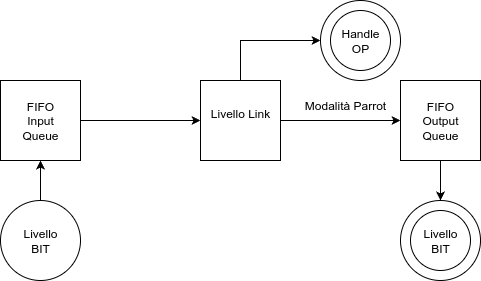
\includegraphics[width=0.5\textwidth]{fifo_input_output.png}
    \caption{Schema del flusso dei pacchetti tra FIFO Input, Livello Link e FIFO Output}
    \label{fig:fifo_input_output}
\end{figure}

\subsection{Gestione dei Token (TKN)}

Un aspetto centrale riguarda la possibilità, per i nodi non-hotspot, di trasmettere i pacchetti contenuti nella propria coda di Output solo quando l’hotspot concede loro un \emph{token} (operazione \texttt{TKN}).  

Quando un nodo riceve un pacchetto \texttt{TKN} in frequenze \emph{master}, acquisisce il diritto di trasmissione per un tempo massimo di \textbf{1 minuto}.  
Durante questo intervallo, il nodo può: 
\begin{itemize}
  \item inviare un pacchetto con operazione \texttt{EXT} per richiedere l’estensione del token. In tal caso l’hotspot risponde con un acknowledgment (\texttt{OP:OK}) e il tempo si prolunga di un ulteriore minuto;
  \item inviare un semplice \texttt{OP:OK} per confermare la gestione del token entro il minuto stabilito.
\end{itemize}

Se entro il tempo limite il nodo non invia alcun messaggio, il token decade automaticamente e l’hotspot lo assegna ad un altro dispositivo.  
È dunque responsabilità del nodo non-hotspot calcolare i tempi necessari per le proprie trasmissioni future e decidere se richiedere estensioni o accordarsi con l’hotspot per la durata del token.  

Questa rappresenta attualmente la parte più delicata del protocollo: al momento della stesura il funzionamento è ancora limitato, ma in prospettiva si prevede la possibilità che anche i nodi non-hotspot possano generare autonomamente token, così da estendere la rete su più livelli e aumentare la flessibilità del sistema.  
Questa apertura costituisce un’opportunità interessante, benché richieda un’implementazione più solida per evitare l’accavallamento di comunicazioni su canali multipli quando più nodi tentano di gestire i token in parallelo.  
\begin{figure}[H]
    \centering
    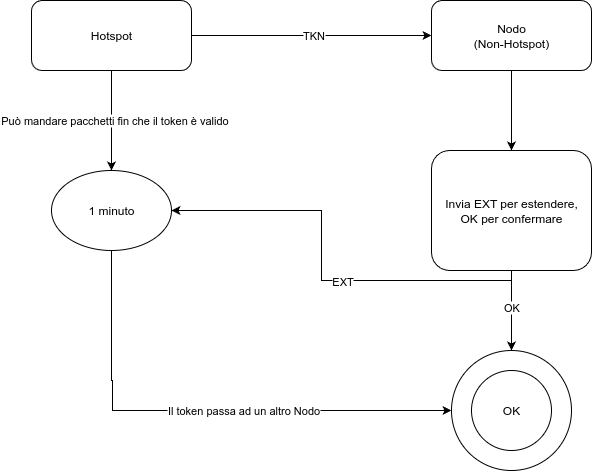
\includegraphics[width=0.65\textwidth]{token_diagram.png}
    \caption{Schema del flusso dei Token tra hotspot e nodi non-hotspot}
    \label{fig:token_diagram}
\end{figure}

\subsection{Comandi di controllo e di rete}

Il Livello Link gestisce alcune operazioni speciali:  
\begin{itemize}
  \item \textbf{ABORT}: comando broadcast (\texttt{ID:1111}) inviato dall’hotspot e ripetuto due volte in frequenze \emph{master} da tutti i nodi non-hotspot. Non richiede ACK e serve a interrompere le operazioni, svuotando i buffer di Input e Output. 
  Viene tipicamente generato quando la piattaforma \emph{Blynk.io} invia il comando \texttt{abort} all’hotspot.
  \item \textbf{OK}: rappresenta l’ACK e viene inviato dai nodi non-hotspot all’hotspot per confermare la ricezione di un pacchetto. 
  Solo in questo momento l’hotspot può eliminare il pacchetto dalla sua coda di Output \emph{master}.
\end{itemize}

Infine, il Livello Link supporta un comando di rete dedicato, \texttt{conns}, che la piattaforma \emph{Blynk.io} invia all’hotspot per ottenere la lista dei nodi attualmente connessi.  

\subsection{Indirizzi di rete}

Gli indirizzi usati dal protocollo sono riassunti nella seguente tabella.  

\begin{table}[H]
\centering
\begin{tabular}{|c|l|}
\hline
\textbf{Indirizzo} & \textbf{Descrizione} \\
\hline
0000 & ID dell'hotspot \\
1111 & Indirizzo broadcast (tutti i nodi) \\
0001 -- 1110 & Range di indirizzi assegnabili ai nodi \\
\hline
\end{tabular}
\caption{Indirizzi di rete del Livello Link}
\label{tab:indirizzi}
\end{table}

\section{Livello Applicazione}
\label{sec:livello_applicazione}
Dato che si conoscono già gli usi futuri di questo protocollo e non è destinato al grande pubblico, 
il dispositivo \textit{hotspot} che riceve in ingresso dal loop \textbf{Blynk} un comando nella forma

\begin{quote}
\texttt{Comando -> IdDestinatario}
\end{quote}

si occupa, con un codice "saldato" al livello Link, sia 
dell'incapsulamento dell'identificativo del destinatario nel formato 
\texttt{ID:IdDestinatario}, sia della traduzione semantica attraverso la seguente tabella. \\
\begin{table}[H]
    \centering
    \label{tab:comandi_hotspot}
    \resizebox{\textwidth}{!}{%
    \begin{tabular}{|l|>{\columncolor{lightgray}}l|l|>{\columncolor{lightgray}}l|}
    \hline
    \textbf{Comando} & \textbf{Operazione} & \textbf{Non-Hotspot} & \textbf{Hotspot} \\
    \hline
    \texttt{movement\_sensor\_on} & \texttt{MOVEMENT\_ON} & 
    \begin{tabular}[c]{@{}l@{}}Esegue misurazione PIR per 5s;\\ restituisce \texttt{MOVEMENT\_YES} o \texttt{MOVEMENT\_NO}\end{tabular} & 
    \texttt{ACK->OP:OK} \\
    \hline
    \texttt{movement\_sensor\_on\_[tempo\_in\_ms]} & \texttt{MOVEMENT\_ON\_[tempo\_in\_ms]} & 
    \begin{tabular}[c]{@{}l@{}}Esegue misurazione PIR per l'intervallo specificato;\\ restituisce \texttt{MOVEMENT\_YES} o \texttt{MOVEMENT\_NO}\end{tabular} & 
    \texttt{ACK->OP:OK} \\
    \hline
    \end{tabular}
    }
    \caption{Mappatura comandi Blynk, operazioni interne e azioni eseguite dai nodi}
\end{table}
Questa tabella mostra come l’hotspot agisca da traduttore e compressore semantico: 
ogni comando testuale viene ridotto a un codice operativo interno e 
ogni dispositivo non-hotspot può eseguire le relative funzioni senza dover 
gestire sintassi testuali complesse. \\ 
Il ritorno dell’esecuzione è anch’esso 
standardizzato (nel caso illustrato, \texttt{MOVEMENT\_YES} / \texttt{MOVEMENT\_NO}), 
mentre l’hotspot conferma localmente con un messaggio di tipo 
\texttt{ACK->OP:OK}, garantendo così sia l’affidabilità della comunicazione 
che la compatibilità futura con ulteriori estensioni già previste.


Quindi l'utente finale che sia l'industria mineraria, soccoritori o tecnici possono 
digitare un comando tramite l'interfaccia \textbf{Blynk.io}, 
corrisponde ad un'\textbf{operazione più compatta} che viene effettivamente interpretata dai nodi della rete. \\
La \textbf{compressione} avviene quindi su due livelli: non solo a livello di codifica dei bit, ma anche a \textbf{livello semantico}, 
poiché i comandi accettati non appartengono a categorie generiche di protocolli di uso comune 
(web come \texttt{HTML/PHP}, o trasferimento file come \texttt{PNG/JPG} nei protocolli \texttt{FTP/HTTP}), 
bensì ad un insieme chiuso e proprietario di istruzioni standardizzate. \\
In questo modo l’interpretazione da parte dei dispositivi risulta rapida e priva di ambiguità, 
mentre l’interfaccia utente mantiene la leggibilità e la semplicità d’uso.

\begin{figure}[H]
    \centering
    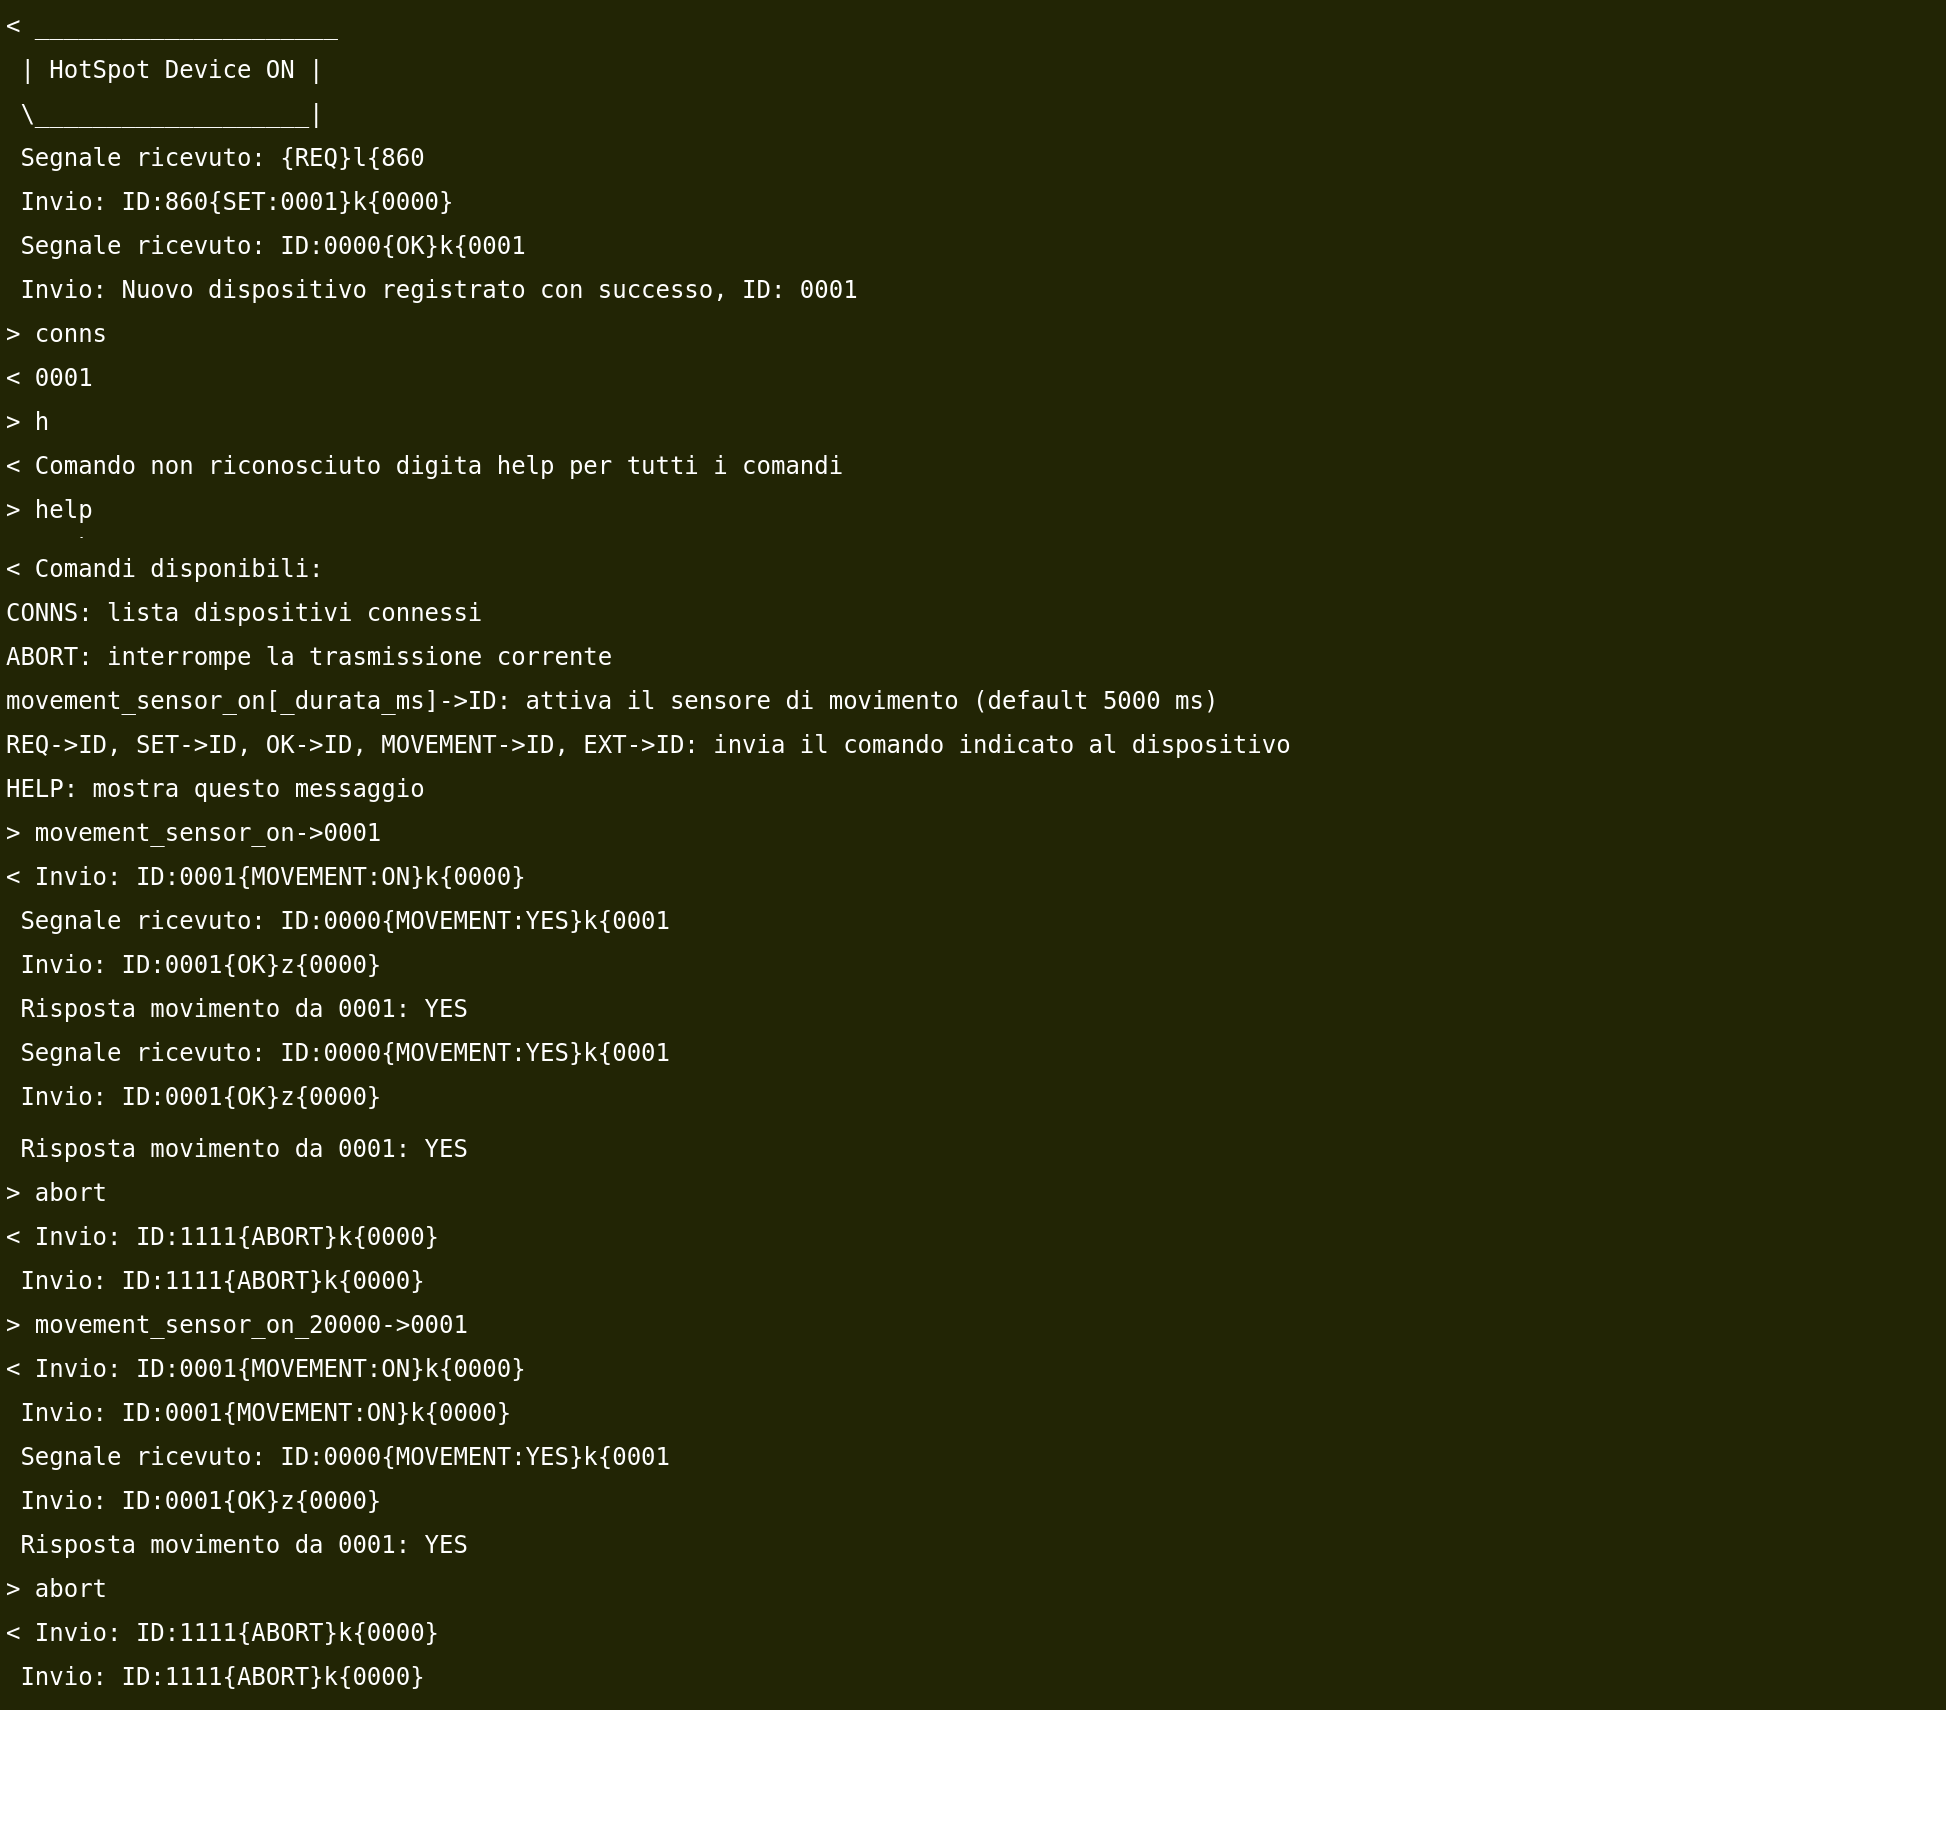
\includegraphics[width=0.80\textwidth]{blynk_interface.png}
    \caption{Utilizzo del Livello Applicazione tramite l'interfaccia Blynk.io}
    \label{fig:blynk_interface}
\end{figure}



